% ------------------------------------------------
%          FILE:  listening.tex
%       CREATED:  Dom 30/Dez/2012 hs 15:59
%   LAST CHANGE:  2013 Mar 28 06:38:22 AM
%        AUTHOR:  Sérgio Luiz Araújo Silva
%          SITE:  http://vivaotux.blogspot.com
%       TWITTER:  @voyeg3r
%         SKYPE:  sergioaraujosilva
% -------------------------------------------------

\chapter{O que você pode ouvir você pode dizer}\label{cha:listening}
\index{Listening}

Desde o início ouça inglês real, desse modo você vai aprender a pronúncia
correta sem que isso seja uma preocupação explícita, se você tiver uma boa
pronúncia significa que você será capaz de discernir melhor os sons dos
falantes nativos do inglês, esse é um dos principais motivos que levam pessoas
que se consideram boas no inglês mas que quando chegam nos EUA ficam
completamente perdidas. O título desta seção foi inspirado em um professor de
inglês chamado \emph{Shane M. Peterson} ou \hypertarget{shane}{coach Shane}
\href{https://twitter.com/coachshane}{@coachshane}, ele atualmente vive na
Coreia do Sul e seu canal no \index{Shane!Youtube}
\href{http://www.youtube.com}{youtube} é:
\href{https://www.youtube.com/user/coachshanesesl}{coachshanesesl} Ele tem
várias séries bem legais para estudantes da lingua inglesa, uma delas chamas-se
\href{https://www.youtube.com/user/dailydictation}{``English
Dictation''}\footnote{https://www.youtube.com/user/dailydictation}, ou ditado
diário de inglês. Do mesmo autor cito a série
\href{ttps://www.youtube.com/user/DailyEasyEnglish}{``DailyEasyEnglish''}\footnote
{https://www.youtube.com/user/DailyEasyEnglish}.

\begin{figure}[h!]
	\centering
	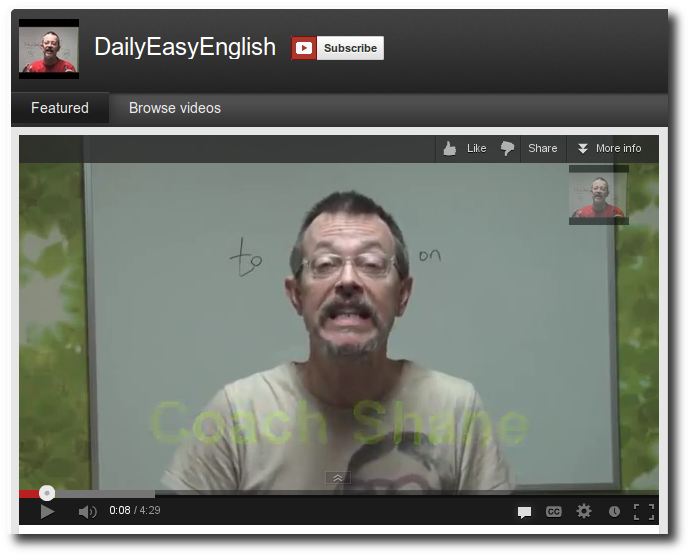
\includegraphics[width=0.8\textwidth]{shane}
	\caption{Coach Shane em uma de suas aulas}
	\index{Shane}
\end{figure}

\noindent Outro professor que tem uma ótima série no youtube é o \index{Teacher
Phill}
\href{https://www.youtube.com/user/TeacherPhilEnglish}{``TeacherPhill''}\footnote{https://www.youtube.com/user/TeacherPhilEnglish}
um de seus canais se chama
\href{https://www.youtube.com/course?list=EC6E296AEDF49E3528}{``Accent Reduction''} e pode ser acessado através deste link:
\href{http://goo.gl/x6SKU}{http://goo.gl/x6SKU} nesta série ele faz a leitura
de um texto e ao final ele fará uma nova leitura mostrando o significado de
algumas palavras e sinônimos.

\vspace{0.3\baselineskip}
\noindent
{\footnotesize \ding{42} ``The great aim of education is not knowledge but action.''
{\em Herbert Spencer} }

\vspace{0.3\baselineskip}
\noindent
{\footnotesize \ding{42} Conheça outros participantes do twitter que postam em inglês na seção
\ref{sec:EnglishLife} página~\pageref{sec:EnglishLife}  }

% tab to continue

\section{Ouça inglês diariamente}\label{sec:ouca}

Ouvir inglês diariamente é uma das principais chaves para atingir a fluência no
inglês, o primeiro passo nessa direção é adquirir um bom
smartphone\footnote{Telefone inteligente} para o qual você deve baixar vários
\index{Podcasts} podcasts e se possível inscreva-se em alguns sites como {\em
twitter} {\em facebook} etc.

Nesta seção você conhecerá alguns links de bons {\em
podcasts}\footnote{Geralmente arquivos em formato mp3 para ouvir em smartphones
e celulares}, ouça inglês pelo menos 30 minutos por dia, para começar um
podcast que é muito bom para iniciantes é o
\href{http://www.eslpod.com/website/index\_new.html}{{\em English as Second Language}}\footnote{http://www.eslpod.com/website/index\_new.html}:
\href{http://goo.gl/Qih6}{http://goo.gl/Qih6} o bom dele é que o audio é lido
pela primeira vez com comentários e de forma bem lenta, certamente você não
compreenderá tudo, mas não se preocupe, em muito pouco tempo você será capaz de
compreende-lo completamente, não tenha tanta pressa.  Outra opção interessante
é o podcast \href{http://edition.englishclub.com/category/listening-news/}{{\em
Listen to the
news}}\footnote{http://edition.englishclub.com/category/listening-news/} no
qual cada audio tem uma transcrição quase completa. Há também um excepcional
podcast intitulado ``culips-english'' que pode ser acessado neste link:
\href{http://esl.culips.com/}{http://esl.culips.com/}, são duas canadenses que
narram histórias muito boas, neste podcast muitas dicas legais, não deixe de
visitar. O site
\href{http://www.bbc.co.uk/portuguese/topicos/aprenda\_ingles/}{``BBC
Brasil''}\footnote{http://www.bbc.co.uk/portuguese/topicos/aprenda\_ingles/}
também tem um acervo bastante interessante neste caso específico você assite
a vídeos nos quais é feita a introdução de novos termos, a história é então
contada e ao final a mesma história é recontada com legendas (Note que
entre os tópicos a serem lidos tem uns com setinhas ``são os vídeos''). Visite
também o site \href{http://www.newsinslowenglish.com/}{\emph{http://www.newsinslowenglish.com/}}.
Neste link do englishclub.com {\footnotesize \ding{42}} \href{http://goo.gl/DkUva}{http://goo.gl/DkUva} você encontrará
dezenas de ditados, ou seja, exercícios para testar
sua capacidade de ouvir.

\vspace{0.3\baselineskip}
\noindent
Um bom canal do \index{VOA!youtube} youtube para quem está começando no inglês
é o \index{VOA} \href{https://www.youtube.com/user/voalearningenglish}{{\em VOA
- Voice of America}}\footnote{https://www.youtube.com/user/voalearningenglish}
pois as notícias lidas nele aparecem com legenda e em 1/3 da
velocidade normal, você pode baixar os videos desse e de outros canais
instalando a extensão video download helper para o firefox à partir deste link:
\href{http://goo.gl/S0xvP}{http://goo.gl/S0xvP} -- {\em link
orignal}\footnote{https://addons.mozilla.org/en-US/firefox/addon/video-downloadhelper}.
\label{Youtube!baixar vídeos} \index{Firefox!video download helper}

\begin{figure}[h!]
	\centering
	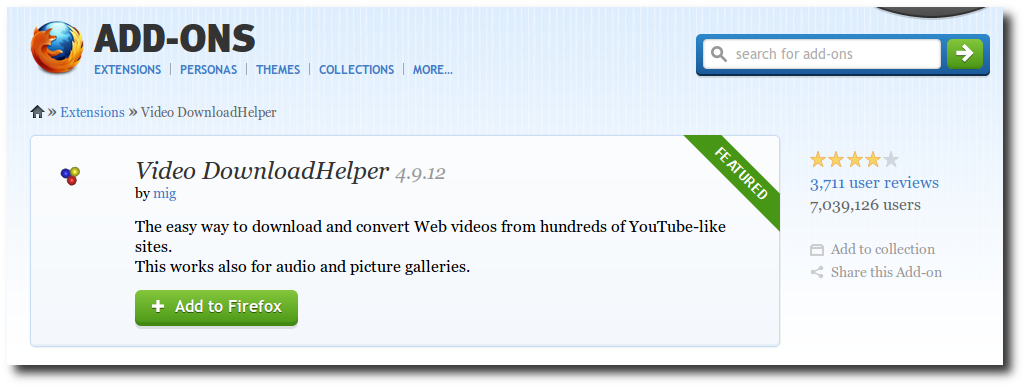
\includegraphics[width=0.8\textwidth]{video-helper}
	\label{img:video-helper}
\end{figure}

\noindent
{\footnotesize \ding{42}  Após instalada a extensão aparecem umas bolinhas coloridas no
lado da barra de endereços do navegador, clicando na setinha ao lado
e escolha a opção ``medium'' que é a de melhor qualidade.}

\vspace{0.3\baselineskip}
\noindent
{\footnotesize \ding{42} Veja também a extensão gtranslate na subseção \ref{sec:google}
na página~\pageref{sec:google}}

\vspace{0.3\baselineskip} \noindent Para usuários Linux há outra opção que permite baixar
playlists do youtube, trata-se do programa
\href{http://rg3.github.com/youtube-dl/}{{\tt
youtube-dl}}\footnote{http://rg3.github.com/youtube-dl/}, no Ubuntu Linux
instale o programa através do comando:\\

{\tt sudo apt-get install youtube-dl \&\& sudo youtube-dl -U}

\vspace{0.3\baselineskip}
\noindent
Para baixar um playlist inteiro faça:\\

{\tt youtube-dl -cit  https://www.youtube.com/user/DailyEasyEnglish}

\section{Como ter vídeos do youtube no celular}
\label{sec:como_ter_v_deos_do_youtube_no_celular}

A extensão \emph{Video Download Helper} citada anteriormente permite baixar
vídeos em formato mp4, \emph{para o caso de aparelhos mais modernos},
mas se você não possui um smartphone, ou seja, tem um celular comum a
extensão lhe permite baixar os vídeos em formato
\emph{3gp}\footnote{https://pt.wikipedia.org/wiki/3GP} , com este
formato você pode ver o vídeo no seu celular, mesmo que ele seja um
aparelho simples.

\begin{figure}[h!]
	\centering
	\caption{Vídeo baixado compatilvel com celulares mais modestos}
	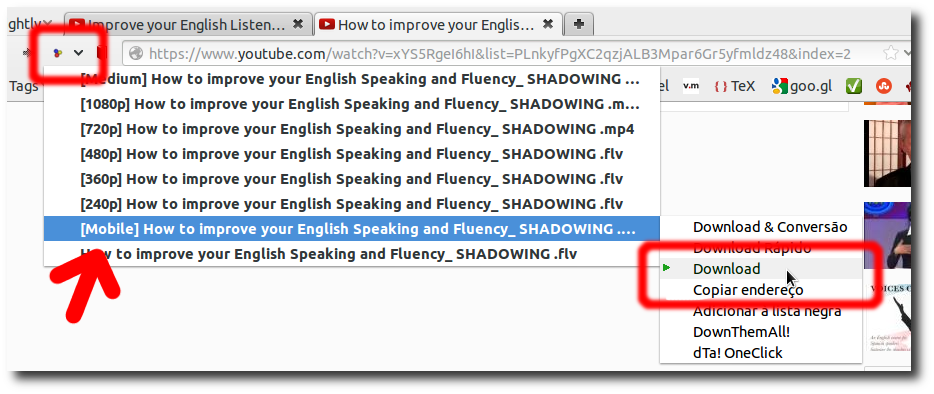
\includegraphics[width=0.8\textwidth]{mobile}
\end{figure}

% section como_ter_v_deos_do_youtube_no_celular (end)

\section{Como melhorar sua capacidade de ouvir}
\label{sec:como_melhorar_sua_capacidade_de_ouvir}

O simples fato de ouvir muito inglês pode não ser suficiente para
garantir uma melhora consistente na sua capacidade de compreensão,
você deve evitar algumas armadilhas. {\footnotesize \ding{42} fonte:
\href{https://www.youtube.com/watch?v=EkxaoaF5wgw}{https://www.youtube.com/watch?v=EkxaoaF5wgw}}.

\begin{description}
	\item[Material muito difícil] e você não entende.
	\item[O material não é interessante para você] e você não se importa.
	\item[É algo chato] e você realmente não quer ouvir.
\end{description}

\dots Se você ouve coisas que tem uma ou mais características acima
é natural que você não se concentre ou absorva o inglês como uma espoja.
Tudo o que você precisa é ouvir conteúdos que são o oposto das características
citadas acima.

\begin{description}
	\item[O material é fácil] e você entende.
	\item[É interessante pra você] e você se importa.
	\item[É excitante] e você quer ouvir.
\end{description}

% section como_melhorar_sua_capacidade_de_ouvir (end)

\section{Os blocos sonoros}\label{sec:blocos-sonoros}

Imagine uma conversação comum do dia-a-dia na qual uma pessoa diz
``você vai mesmo?'', na verdade a palavra {\em você} muitas vezes
transforma-sem em {\em cê} e a palavra {\em mesmo} transforma-se em
{\em mêz}, temos então um grande bloco sonoro, com todos os fonemas
ligados mais ou menos assim: ``cêvaimês.'' No idioma inglês acontece
exatamente a mesma coisa, os sons são abreviados (principalmente
quando se fala rápido) e além disso acontecem as ligações sonoras que
em inglês chamam-se {\em linking words}, {\em reductions} ou ainda
morphing, por exemplo na lingua escrita, ou nos livros formais é comum algo do tipo:
\underline{{\em I wanto to buy a car}}, mas no inglês falado a coisa fica assim:
{\em  \underline{I \textcolor{red}{wanna} buy a car}}. Veja este outro trecho:
\emph{\textcolor{red}{whatcha} thinking?} sua escrita longa em inglês fica assim \emph{What you are thinking?}
Ao trabalhar a audição (listening) trabalhe sempre prestando atenção em como as palavras são
abreviadas e como seus sons estão conectados, isso explica em parte o
fato de estudantes que se consideram avançados no Brasil não
conseguirem se comunicar por exemplo em uma viagem aos Estados Unidos,
é que no seu método de estudo, geralmente baseado na lingua formal não
é visto nada a respeito da sonoridade coloquial, ou seja, do inglês do
dia-a-dia.

\vspace{0.5cm}
{\footnotesize \ding{42}  have a lo\textcolor{red}{t t}o study for the next test.}
\vspace{0.5cm}

\noindent
Existe uma diferença entre a lingua escrita como por exemplo em ``What you do?'',
em relação ao mesmo trecho pronunciado no dia-a-dia ``Wharia do?''
\vspace{0.5cm}

\noindent
Para completar a compreensão dos blocos sonoros o estudante deverá conhecer os
{\em Slangs} que são as gírias, os provérbios e os {\em phrasal verbs}, que são
duas ou mais palavras combinadas que ganham novo sentido devido o contexto em
que se encontram.  Pra finalizar, tenha consciência que você deverá buscar
conversas reais, de falantes nativos, pois a pronúncia e a entonação são
naturalmente corretos. Lembre-se se você conviver com quem tem uma pronúncia
ruin ou não totalmente perfeita você tenderá naturalmente a reproduzir seus
erros. Para aprender mais como combinar palavras veja as lições do
professor \hyperlink{shane}{Shane} no capítulo \ref{cha:listening} página~\pageref{cha:listening}.

\subsubsection{Não estude pronúncia de palavras isoladas}

O contexto também determina a pronúncia de certas palavras, portanto tentar
aprender a pronúncia de palavras isoladas não lhe dará a habilidade de ouvir ou
pronunciar inglês real. Por exemplo a palavra ``to'', em algumas frases ela
muda completamente a sonoridade para algo como: ``I’m going {\bf tuh} the
store.'' \\
{\footnotesize \ding{42}  Para mais detalhes veja:
\href{http://www.englishanyone.com/index.php?page=jsbo3day2}{www.englishanyone.com}\footnote{http://www.englishanyone.com/index.php?page=jsbo3day2}.}

\noindent
{\footnotesize \ding{42} Um bom site para aprimorar sua pronúncia é o \href{http://pt.englishcentral.com}{http://pt.englishcentral.com}}

\section{Lista de podcasts}
\label{sec:lista_de_podcasts}

\begin{verbatim}
http://elllo.org/
http://www.lyricstraining.com/index.php
http://www.listen-to-english.com/
http://www.learnglish.net/
http://www.audiopuzzler.com/index.html
http://www.listen-and-write.com/
http://accent.gmu.edu/index.php (for getting used to different accents)
http://reallifebh.com/real-life-english-esl-podcasts
\end{verbatim}

% section lista_de_podcasts (end)

% Alguns exemplos com frases reais, do dia a dia:
% \begin{verbatin}
% How ya doin?
% What ya doin today
% I ma fa nof baseball
% \end{verbatin}
